%% LyX 2.0.3 created this file.  For more info, see http://www.lyx.org/.
%% Do not edit unless you really know what you are doing.
\documentclass[oneside,spanish]{book}
\usepackage[T1]{fontenc}
\usepackage[latin9]{inputenc}
\usepackage{listings}
\usepackage[a4paper]{geometry}
\geometry{verbose,tmargin=3cm,bmargin=3cm,lmargin=3cm,rmargin=4cm}
\usepackage{fancyhdr}
\pagestyle{fancy}
\setcounter{secnumdepth}{3}
\setcounter{tocdepth}{3}
\usepackage{longtable}
\usepackage{pifont}
\usepackage{textcomp}
\usepackage{amstext}
\usepackage{graphicx}

\makeatletter

%%%%%%%%%%%%%%%%%%%%%%%%%%%%%% LyX specific LaTeX commands.
\newcommand{\noun}[1]{\textsc{#1}}
%% Because html converters don't know tabularnewline
\providecommand{\tabularnewline}{\\}

%%%%%%%%%%%%%%%%%%%%%%%%%%%%%% Textclass specific LaTeX commands.
\newenvironment{lyxcode}
{\par\begin{list}{}{
\setlength{\rightmargin}{\leftmargin}
\setlength{\listparindent}{0pt}% needed for AMS classes
\raggedright
\setlength{\itemsep}{0pt}
\setlength{\parsep}{0pt}
\normalfont\ttfamily}%
 \item[]}
{\end{list}}

%%%%%%%%%%%%%%%%%%%%%%%%%%%%%% User specified LaTeX commands.
\usepackage[T1]{fontenc}
\usepackage[spanish]{babel}
\usepackage{times}

\usepackage{color}
\definecolor{gray97}{gray}{.97}
\definecolor{gray75}{gray}{.75}
\definecolor{gray45}{gray}{.45}

\usepackage{listings}
\lstset{ %
language=C++,
frame=single,
%frame=Ltb,
%framerule=0pt,
%aboveskip=0.5cm,
%framextopmargin=3pt,
%framexbottommargin=3pt,
%framexleftmargin=0.4cm,
%framesep=0pt,
%rulesep=.4pt,
%backgroundcolor=\color{gray97},
rulesepcolor=\color{black},
stringstyle=\ttfamily,
showstringspaces = false,
basicstyle=\small\ttfamily,
commentstyle=\color{gray45},
keywordstyle=\bfseries,
numbers=left,
%numbersep=15pt,
numbersep=5pt,
%numberstyle=\tiny,
%numberfirstline = false,
breaklines=true,
}

\AtBeginDocument{
  \def\labelitemi{\Pisymbol{psy}{183}}
  \def\labelitemii{\(\diamond\)}
}

\makeatother

\usepackage{babel}
\addto\shorthandsspanish{\spanishdeactivate{~<>}}

\begin{document}

\title{USACO Training Book}


\author{Autor}


\date{25 de Agosto de 2013}

\maketitle
\tableofcontents{}


\chapter{Primeros Pasos}


\section*{Tipos de Problemas de Competencias de Programación}

Hal Burch condujo un análisis durante el receso de primavera de 1999
e hizo un descubrimiento asombroso: ¡Solo hay 16 tipos de problemas
de competencias de programación! Aún más, los primeros cubren casi
el 80\% de los problemas vistos en la IOI. Ellos son:
\begin{itemize}
\item Programación Dinámica
\item Avaro
\item Bùsqueda Completa
\item Llenado Por Inundación
\item Camino Mas Corto
\item Técnicas de Bùsquedas Recursivas
\item Arbol de Minima Expansión
\item Mochila
\item Geometría computacional
\item Flujo de Redes
\item Camino Euleriano
\item Envolvente convexa bidimensional
\item Numeros Grandes
\item Busqueda Heurística
\item Busqueda Aproximada
\item Problemas Ad Hoc
\end{itemize}
Los problemas más desafiantes son Problemas Combinados los cuales
involucran un ciclo (combinaciones, subconjuntos, etc.) alrededor
de uno de los algoritmos antes mencionados - o aún un ciclo de un
algoritmo con otro dentro de él. Estos parecen extraordinariamente
difíciles para tener correctos, aunque conceptualmente son ``obvios''.

Si usted puede dominar 40\% de estos tipos de problemas, se le puede
casi garantizar a usted una medalla de plata en la IOI. Dominar el
80\% lo promueve en el rango oro casi seguro. Por supuesto, ¡`dominar`
es una nuez difícil de romper! Le daremos bastantes problemas de tal
manera que usted pueda mejorar sus habilidades en su búsqueda por
fama internacional. 


\section{Problemas Ad Hoc}

Los problemas ``Ad hoc'' son aquellos cuyos algoritmos no caen en
ninguna categoria estandar con soluciones bien-estudiadas. Cada problema
ad hoc es diferente; no existen técnicas generales o especifícas para
resolverlos.

Por supuesto, esto hace que esos problemas sean los `divertidos',
ya que cada uno presenta un nuevo desafío. Las soluciones podrían
requerir una estructura novedosa o un conjunto inusual de ciclos o
condicionales. Algunas veces ellos requieren combinaciones especiales
que son raras, o al menos raramente encontradas.

Los problemas ad hoc usualmente requieren lectura cuidadosa y usualmente
conducen a un ataque que se revuelve alrededor de una secuencia cuidadosa
de las instrucciones dadas en el problema.

Los problemas ad hoc pueden aún requerir optimizaciones razonables
y al menos un grado de análisis que le permita a uno evitar ciclos
anidados cinco veces, por ejemplo.

En esta página aparecen más problemas ad hoc que otros tipos de problemas.
Siempre esté listo para un problema ad hoc si usted no puede clasificar
un problema como uno de los otros tipos estandar (a ser listados después). 


\section{Búsqueda Completa }


\subsection{La Idea}

Resolver un problema usando búsqueda completa se basa en el principio
\textquotedbl{}Mantengálo Simple\textquotedbl{}. El propósito de resolver
problemas de competencia es escribir programas que corran en el tiempo
permitido, independientemente que haya un algoritmo más rápido.

La Busqueda Completa explota el metodo de fuerza bruta, líneal, trate-todos.
Este método debería ser siempre el primer algoritmo/solución que usted
debe considerar. Si esto trabaja dentro de las restricciones de tiempo
y de espacio, entonces hagálo: es fácil de codificar y usualmente
fácil de depurar. Esto significa que usted tendrá más tiempo para
trabajar en los problemas dificiles, en los que la fuerza bruta no
trabaje lo suficientemente rápido.

En el caso de un problema con solo menos de un par de millones de
posibilidades, itere en cada una de ellas, y vea si la respuesta funciona.


\subsection*{Cuidado, Cuidado}

Algunas veces no es obvio que usted use esta metodología.


\subsection*{Problema: Lamparas de Fiesta {[}IOI 98{]}}

A usted se le dan N lamparas y cuatro interruptores. El primer interruptor
maneja todas las lámparas, el segundo las pares, el tercero las impares,
y el último las lámparas 1, 4, 7, 10, ...

Dados el número de lámparas, N, el número de veces en que se ha presionado
un botón (hasta 10,000), y el estado de algunas de las lámparas (por
ejemplo la lámpara 7 está apagada), dé como salida todos los posibles
estados en que podrían estar las lámparas.

Candidamente, para cada presión de botón, usted debe considerar 4
posiblidades, para un total de 410000 (aproximadamente 106020 ), lo
que significa que no hay manera en que usted podría hacer búsqueda
completa (este algoritmo haría explotar la recursión).

Teniendo en cuenta que el orden de las presiones de botón no interesa
se baja este número a cerca de 100004 (aproximadadmente 1016 ), aún
un número demasiado grande para hacer búsqueda completa (pero ciertamente
más cercano por un factor sobre 106000 ).

Sin embargo, presionar un botón dos veces es lo mismo que presionar
el botón ninguna vez, por lo tanto todo lo que usted debe verificar
es si cada botón se presionó 0 o 1 veces. Esto es solo 24 = 16 posibilidades,
seguro un número de iteraciones resoluble dentro del límite de tiempo.


\subsection*{Problema 3: Los Relojes {[}IOI 94{]}}

Un grupo de nueve relojes habita en una grilla 3 x 3; cada uno marca
las 12:00, las 3:00, las 6:00, o las 9:00. Su objetivo es manipularlos
para que todos marquen 12:00. Desafortunadamente, la única manera
en que usted puede manipular los relojes es por uno de nueve tipos
diferentes de movimientos, cada uno de los cuales rota cierto subconjunto
de los relojes 90 grados en sentido horario.

Encuentre la secuencia más corta de movimientos que pongan todos los
relojes a las 12:00.

La cosa ''obvia'' es hacer una solución recursiva, la cual verifica
si hay una solución de 1 movimiento, 2 movimientos, etc. hasta que
encuentre una solución. Esto tomaria 9k tiempo, donde k es el número
de movimientos. Desde que k podría ser muy grande, esto no correría
razonablemente dentro de las limitaciones de tiempo.

Note que el orden de los movimientos no interesa. Esto reduce el tiempo
a k9 , lo cual no es una mejora suficientemente buena.

Sin embargo, desde que hacer cada movimiento 4 veces es lo mismo que
hacerlo ninguna vez, usted sabe que ningún movimiento será hecho más
de 3 veces. Por lo tanto únicamente hay 49 posibilidades, lo cual
es solamente 262,072, el cual, dada la regla de correr más de 10,000,000
operaciones en un segundo, debería trabajar en tiempo. La solución
a fuerza bruta, teniendo en cuenta estas cosas, es adecuada perfectamente.


\subsection{Problemas Ejemplo}


\subsubsection*{Vacas Lecheras {[}Ronda de Competencia de la USACO 1996{]}}

Dado un horario de ordeño (El Granjero A ordeña de las 3:00 a las
10:00, El Granjero B de 7:00 a 12:00, etc.), calcule
\begin{itemize}
\item El intervalo más largo de tiempo en que al menos una vaca está siendo
ordeñada
\item El intervalo más largo de tiempo en que ninguna vaca está siendo ordeñada 
\end{itemize}

\subsubsection*{Vacas Perfecas Y Vacas Primas Perfectas}

Un número perfecto es aquel cuya suma de los divisores propios es
igual al número. Por ejemplo, 28 = 1 + 2 + 4 + 7 + 14. Un par perfecto
es un par de números tales que la suma de los divisores propios de
cada uno es igual al otro. Hay, por supuesto, conjuntos perfectos
más grandes, tales que la suma de los divisores del primero es igual
al segundo, la de los divisores del segundo es igual al tercero, etc.,
hasta que la suma de los divisores propios del último es igual al
primer número.

A cada vaca en el rancho del Granjero Juan se le asigna un número
serial, de 1 a 32000. Una vaca perfecta es aquella que tiene asignado
un número perfecto como su serial. Un grupo de vacas es un conjunto
de vacas primas perfectas si sus numeros seriales forman un conjunto
perfecto. Encuentre todas las vacas perfectas y todas las vacas primas
perfectas.


\section{Algoritmos Avaros }


\subsubsection*{Problema Ejemplo: Reparación de Establo {[}Abierto de Primavera de
la USACO 1999{]}}

Hay una lista larga de pesebreras, algunas de las cuales necesitan
ser cubiertas con tableros. Usted puede usar hasta N (1 <= N <= 50)
tableros, cada uno de los cuales puede cubrir cualquier número de
pesebreras consecutivas. Cubra todas las pesebreras que haga falta
cubrir, cubriendo tan pocas pesebreras como sea posible.


\subsection{La Idea}

La idea básica detrás de un algoritmo avaro es construir soluciones
más grandes a partir de soluciones más pequeñas. De manera diferente
a otros enfoques, sin embargo, los algoritmos avaros mantienen únicamente
la mejor solución encontrada conforme ellos van avanzando. Por lo
tanto, para el ejemplo problema, para construir la respuesta para
N = 5, ellos encuentran la mejor solución para N = 4, y luego la alteran
para obtener una solución para N = 5. No se considera ninguna otra
solución para N = 4.

Los algoritmos avaros son \emph{rápidos}, generalmente de lineales
a cuadráticos y requieren poca memoria extra. Desafortunadamente,
ellos usualmente no son correctos. Pero cuando funcionan, son frecuentemente
fáciles de implementar y lo suficientemente rápidos para ejecutar.


\subsubsection*{Problemas}

Hay básicamente dos problemas con los algoritmos avaros.


\subsubsection*{Como Construir}

¿Cómo se crea una solución más grande a partir de pequeñas? En general,
esta es una función del problema. Para el problema ejemplo, la manera
más obvia de ir de cuatro tableros a cinco es elegir un tablero y
remover una sección, obteniendo por lo tanto dos tableros a partir
de uno. Usted debería elegir remover la sección más grande de cualquier
tablero que cubra solo pesebreras que no necesiten ser cubiertas (minimizando
por lo tanto el número total de pesebreras cubiertas).

Para remover una sección de pesebreras cubiertas, tome el tablero
que cubre esas pesebreras, y conviertalo en dos tableros: uno de los
cuales cubre las pesebreras antes de la sección, el otro cubre las
pesebreras después de la sección

¿Sirve?

El desafío real para el programador cae en el hecho que las soluciones
avaras no siempre sirven. Aún si parecen funcionar para las entradas
ejemplo, entradas aleatorias, y todos los casos que usted pueda pensar,
si hay un caso donde no trabaje, al menos uno (¡si no más!) de los
casos de prueba del jurado serán de esa forma.

Para el problema ejemplo, para ver si el algoritmo avaro antes descrito
sirve, considere lo siguiente:

Asuma que la respuesta no contiene el hueco grande que el algoritmo
removió, pero contiene un hueco que es menor. Combinando los dos tableros
en los extremos del hueco más pequeño y partiendo el tablero a través
del hueco más grande, se obtiene una respuesta que usa tantos tableros
como la solución original pero el cual cubre menos pesebreras. Esta
nueva respuesta es mejor, por lo tanto la asunción está errada y deberiamos
elegir siempre remover el hueco más grande.

Si la respuesta no contiene este hueco en particular, pero contiene
otro hueco el cual es tan grande, haciendo la misma transformación
se tiene una respuesta que usa el mismo número de tableros y cubre
tantas pesebreras como la otra respuesta. Esta nueva respuesta es
tan buena como la solución original, pero no mejor, por lo tanto podemos
elegir cualquiera.

Por lo tanto, existe una respuesta óptima la cual contiene el hueco
grande, entonces, en cada paso, hay siempre una solución óptima la
cual es un superconjunto del estado actual. Por lo tanto, la solución
final es óptima.


\subsubsection*{Conclusiones}

Si existe una solución avara, uséla. Son fáciles de codificar, fáciles
de depurar, corren rápido, y usan poca memoria, definen básicamente
un algoritmo en términos de competencia. El único elemento faltante
de esta lista es correctitud. Si el algoritmo avaro encuentra la solución
correcta, uselo, pero no se engolosine pensando que la solución avara
trabajará para todos los problemas.


\subsection{Problemas Ejemplo}


\subsubsection*{Ordenando una secuencia de tres valores {[}IOI 1996{]}}

A usted se le da una secuencia de tres valores (1, 2, o 3) de longitud
hata 1000. Encuentre el mínimo número de intercambios para poner la
secuencia en orden.
\begin{description}
\item [{Algoritmo:}] La secuencia tiene tres partes: la parte que estará
llena de 1`s cuando esté ordenada, la parte que estará llena de 2`s
cuando esté ordenada y la parte que estará llena de 3`s cuando esté
ordenada. El algoritmo avaro intercambia tantos 1`s en la parte 2
con los 2\textasciiacute{}s en la parte 1 como sea posible, tantos
1`s en la parte 3 con 3\textasciiacute{}s en la parte 1 como sea posible,
y 2\textasciiacute{}s en la parte 3 con 3`s en la parte 2. Una vez
que no quedan ninguno de estos tipos, los elementos restantes fuera
de lugar necesitan ser rotados de una manera u otra en conjuntos de
3. Usted puede ordenar optimamente estos intercambiando todos los
1\textasciiacute{}s hacia su lugar y luego los 2`s.
\item [{Análisis:}] Obviamente, un intercambio puede poner a lo más dos
elementos en su lugar, por lo tanto todos los intercambios del primer
tipo son óptimos. Tambièn, es claro que ellos usan diferentes tipos
de elementos, por lo tanto no hay ''interferencia'' entre esos tipos.
Esto implica que el orden no interesa. Una vez que estos intercambios
han sido ejecutados, lo mejor que usted puede hacer es dos intercambios
por cada tres elementos que no estén en la ubicación correcta, lo
cual es lo que la segunda parta obtendrá (por ejemplo, ùnicamente
todos los 1\textasciiacute{}s son puestos en su lugar; luego todos
los 2`s restantes en el lugar de los 3`s y viceversa, y los que puedan
ser intercambiados).
\end{description}

\subsubsection*{Monedas Amigas - Un Contraejemplo {[}abreviado{]}}

Dadas las denominaciones de monedas de un pais recientemente fundado,
el País Lechero, y una cantidad monetaria, encuentre el conjunto de
monedas más pequeño que sume esa cantidad. Se garantiza que el País
Lechero tendrá la moneda de 1 centavo.
\begin{description}
\item [{Algoritmo:}] Use la moneda con valor más alto que no sea mayor
que el objetivo e itere en el total menos el monto obtenido con esa
moneda.
\item [{Análisis}] (incorrecto): Obviamente, usted nunca quiere usar un
valor más pequeño de moneda, pues eso implicaría que usted tiene que
usar más monedas para hacer la diferencia, por lo tanto este algoritmo
sirve.
\item [{Tal}] vez no: Bien, el algoritmo usualmente funciona. De hecho,
para el sistema de monedas norteamericano \{1, 5, 10, 25\}, siempre
da el conjunto óptimo. Sin embargo, para otros conjuntos, como \{1,
5, 8, 10\} y un objetivo de 13, este algoritmo avaro daría un 10,
y luego tres 1`s, para un total de cuatro monedas, cuando también
existe la solución con dos monedas \{5, 8\}.
\end{description}

\subsubsection*{Orden Topológico}

Dada una colección de objetos, junto con algunas restricciones de
orden, tales como \textquotedbl{}A debe ir antes que B\textquotedbl{}
encuentre un orden de los objetos tal que se cumplan las restricciones
de orden.
\begin{description}
\item [{Algoritmo:}] Cree un grafo directo sobre los objetos, donde hay
un arco de A a B si \textquotedbl{}A debe ir antes que B\textquotedbl{}.
Haga una pasada sobre los objetos en orden arbitrario. Cada vez que
usted encuentre un objeto con grado-de-entrada de 0, avaramente pongàlo
al final del ordenamiento actual, borre todos sus arcos de salida,
y ejecute el mismo procedimiento en sus ex hijos. Si este algoritmo
recorre todos los objetos sin poner cada objeto en el orden, no hay
un orden que satisfaga las restricciones. 
\end{description}

\section{Creando Soluciones Ganadoras}

Una buena manera de obtener destreza competitiva es escribir un plan
de acción para lo que usted va a estar haciendo durante una competencia.
Esto lo ayudará a tener un guión para sus acciones, en términos de
que hacer tanto cuando las cosas van bien como cuando van mal. De
esta manera usted puede gastar su tiempo de pensar en la competencia
pensando en problemas de programación y no tratando de imaginarse
que diablos usted debería hacer después... es como precalcular sus
reacciones para la mayoría de las situaciones.

La preparación mental también es importante.


\subsection{Plan de Acción para Una Ronda de Competencia}

Lea \noun{PRIMERO} completamente \noun{TODOS} los problemas; use lápiz
y papel para hacer notas con algoritmos, complejidad, los números,
estructuras de datos, detalles tramposos, ...
\begin{itemize}
\item Imagínese muchos algoritmos posibles - ¡Luego elija el más tonto que
funcione!
\item ¡\noun{HAGA LAS MATEMATICAS}! (complejidad de espacio y de tiempo,
y calcule los números de tiempo esperado y caso peor) 
\item Trate de quebrar el algoritmo - use casos de pruebas especiales (¿degenerados?) 
\item Ordene los problemas: los de trabajo más corto primero, en términos
de su esfuerzo (del más corto al más largo: hecho antes, fácil, no
familiar, difícil)
\end{itemize}
Codificando un problema - Para cada uno, uno a la vez:
\begin{itemize}
\item Termine el Algoritmo 
\item Cree datos de prueba para casos tramposos 
\item Escriba las estructuras de datos Codifique la rutina de entrada y
pruébela (¿escribir rutinas de salida extras para mostrar los datos
?) 
\item Codifique la rutina de salida y pruébela 
\item Refinamiento por Pasos: escriba comentarios que describan la lógica
del programa
\item Llene el código y depure una sección cada vez 
\item Hágalo trabajar y verifique el código funcione adecuadamente (use
casos triviales de prueba) 
\item Trate de quebrar el código - use casos especiales para verificar que
el código funcione adecuadamente
\item Haga optimización progresivamente - solo tanto como sea necesario
y tenga todas las versiones (use casos difíciles para calcular tiempo
actual de corrida)
\end{itemize}

\subsection{Estrategia de manejo de tiempo y Escenarios de \textquotedbl{}control
de daños\textquotedbl{}}

Tenga un plan para que hacer cuando varias cosas (¡previsibles!) vayan
mal; imagine problemas que usted podría tener e imagínese como va
usted a reaccionar. La pregunta central es: \textquotedbl{}¿cuando
usted gasta más tiempo depurando un programa y cuando usted corrige
sus daños y sigue adelante?\textquotedbl{}. Considere estos aspectos:
\begin{itemize}
\item ¿Cuánto tiempo ha usted ya gastado depurando?
\item ¿Qué tipo de error parece que tiene usted?
\item ¿Es su algoritmo incorrecto? 
\item ¿Sus estructuras de datos necesitan ser cambiadas? 
\item ¿Tiene alguna pista de qué anda mal? 
\item Cierta cantidad (20 minutos) de depuración es mejor que cambiarse
a cualquier otra cosa; pero usted debería ser capaz de resolver otro
problema de la nada en 45 minutos. 
\item ¿Cuándo regresar a un problema que abandonó previamente? 
\item ¿Cuándo gastar más tiempo optimizando un programa, y cuando cambiar? 
\item Considere que hacer de aquí en adelante - olvídese del esfuerzo previo,
enfóquese en el futuro: ¿Cómo puede usted obtener más puntos en la
siguiente hora que tiene? 
\end{itemize}
Haga una lista de puntos a hacer antes de enviar sus soluciones:
\begin{itemize}
\item ¿Parar la codificación cinco minutos antes del fin de la competencia?
\item Quite los \textquotedbl{}asserts\textquotedbl{}.
\item Quite toda la salida de depuración
\end{itemize}

\subsection{Sugerencias y Trucos}
\begin{itemize}
\item Use fuerza bruta cuando se pueda !
\item Lo simple es inteligente! Sugerencia: tenga cuidado con los limìtes
(especificados en el enunciado del problema)
\item Gaste memoria cuando esto hace más fácil su vida (si puede hacer realmente
algo con esto) 
\item No borre su salida extra de depuración, póngala como comentario 
\item Optimice progresivamente, y solo tanto como sea necesario
\item ¡Mantenga todas las versiones que funcionen!
\item Codifique para depurar:

\begin{itemize}
\item usar espacios en blanco está bien
\item use nombres de variables que tengan sentido
\item no reutilice variables
\item refinamiento por pasos
\item COMENTE ANTES DE CODIFICAR.
\end{itemize}
\item Evite punteros si puede 
\item Evite usar memoria dinámica como si fuera una plaga: ubique todo estáticamente. 
\item Trate de no usar punto flotante; si tiene que hacerlo, ponga tolerancias
en todo (nunca pruebe igualdad)
\item Comentarios sobre comentarios:

\begin{itemize}
\item No use una larga prosa, solamente notas pequeñas
\item Explique la funcionalidad en alto-nivel : ++i; /{*} aumenta el valor
de i {*}/ es más que inútil 
\item Explique el código que use trucos 
\item Delimite y documente secciones funcionales 
\item Comente como si fuera para alguien inteligente quien conoce el problema,
pero no el código 
\item Comente cualquier cosa que tenga que pensar 
\item Comente cualquier cosa que usted mire más de una vez diciendo, \textquotedbl{}¿Que
hace esto otra vez?\textquotedbl{} 
\item Siempre comente el orden de los índices de arreglos 
\end{itemize}
\item ¡Mantenga un registro de su desempeño en cada competencia: sucesos,
errores, y que podría haber hecho mejor; use esto para re-escribir
y mejorar su plan de juego!
\end{itemize}

\subsection{Complejidad}


\subsubsection*{Bases y Notación de Orden}

La base fundamental del análisis de complejidad gira alrededor la
noción de la notación ''gran O'', por ejemplo: $O(N)$. Esto significa
que la velocidad de ejecución del algoritmo o su uso de memoria se
duplicará cuando el tamaño del problema se duplique. Un algoritmo
de $O(N\text{\texttwosuperior})$ correrá cuatro veces más despacio
(o usará 4 veces más espacio) cuando el tamaño del problema se duplique.
Los algoritmos constantes en tiempo o en espacio se denotan por $O(1)$.
Este concepto se aplica tanto a tiempo como a espacio; aquí nos concentraremos
discutiendo en el tiempo.

Uno deduce el tiempo $O()$ de un programa examinando sus ciclos.
El ciclo más anidado (y por lo tanto más lento) domina el tiempo de
corrida y es el único mencionado cuando se discute notación $O()$.
Un programa con un solo ciclo y un ciclo anidado (presumiblemente
cada uno de los ciclos se ejecutan $N$ veces cada uno) es $O(N\text{\texttwosuperior})$,
aunque sin embargo hay también un ciclo $O(N)$ presente.

Por supuesto, la recursión también cuenta como un ciclo y los programas
recursivos pueden tener ordenes como $O(b^{N})$, $O(N!)$, o aun
$O(N^{N})$.


\subsubsection*{Reglas Prácticas}
\begin{itemize}
\item Cuando analice un algoritmo para tener una idea de cuánto tiempo podría
tomar para un conjunto dado de entrada, la primera regla práctica
es: los computadores modernos (2004) pueden manejar 100M acciones
por segundo. En un limite de cinco segundos para un programa, se pueden
manejar unas 500M acciones. Programas realmente bien optimizados podrían
ser capaces de duplicar o aún cuadruplicar ese número. Los algoritmos
desafiantes podrían únicamente ser capaces de manejar la mitad de
eso. Las competencias actuales usualmente tienen un límite de tiempo
de 1 segundo para grandes conjuntos de datos. 
\item 16MB máximo de memoria para usar 
\item $2^{10}$\textasciitilde{}aproximadamente\textasciitilde{} $10^{3}$
\item Si usted tiene k ciclos anidados corriendo cada uno N iteraciones,
el programa tiene complejidad $O(N^{k})$. 
\item Si su programa es recursivo con b llamadas recursivas por nivel y
tiene $l$ niveles, el programa tiene complejidad $O(b^{l})$. 
\item Tenga en cuenta que hay N! permutaciones y $2^{n}$ subconjuntos o
combinaciones de N elementos cuando se trabaja con esas clases de
algoritmos.
\item Los mejores tiempos para ordenar N elementos son $O(NlogN)$.
\item \noun{¡HAGA LAS MATEMATICAS!} Encadene los números.
\end{itemize}

\subsubsection*{Ejemplos}
\begin{itemize}
\item Un solo ciclo con N iteraciones es $O(N)$: 
\end{itemize}
\begin{lstlisting}
sum = 0
for i = 1 to n
  sum = sum + i
\end{lstlisting}


Un ciclo doblemente anidado frecuentemente es $O(N^{2})$: 

\begin{lstlisting}
# fill array a with N elements
for i = 1 to n-1 
  for j = i + 1 to n 
    if (a[i] > a[j])
       swap (a[i], a[j])
\end{lstlisting}


Note que aunque este ciclo ejecuta $Nx(N+1)/2$ iteraciones de la
sentencia if, es $O(N^{2})$ debido a que duplicar $N$ cuadruplica
los tiempos de ejecución.

Considere este árbol binario bien balanceado con cuatro niveles: 

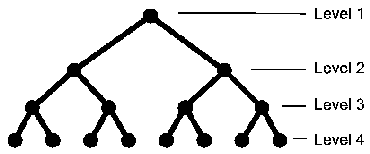
\includegraphics{imagenes/craft1}

Un algoritmo que recorra un arbol binario en general tendrá complejidad
$O(2^{N})$.


\subsection{Paradigmas de Solución}


\subsubsection*{Generando vs. Filtrando}

Los programas que generan montones de respuestas posibles y luego
eligen las que son correctas (imagine el solucionador de 8-reinas)
son filtros. Aquellos que dan exactamente la respuesta correcta sin
comienzos falsos son generadores. Generalmente, los filtros son más
fáciles (más rápidos) de codificar y corren más lentamente. Haga las
matemáticas para ver si son los suficientemente buenos o si necesita
crear y probar un generador.


\subsubsection*{Precálculo}

Algunas veces es útil generar tablas u otras estructuras de datos
que permitan la búsqueda más rápida posible de un resultado. Esto
es llamado precálculo (en el cual uno intercambia espacio por tiempo).
Uno podría compilar datos precalculados en un programa, calcularlo
cuando el programa comience, o simplemente recordarlos cuando los
calcula. Un programa que debe pasar letras de mayúscula a minúscula
cuando están en mayúsculas puede hacer una tabla muy rápida de búsqueda
que no requiera condicionales, por ejemplo. Los programas de competencia
frecuentemente usan números primos - muchas veces es práctico generar
una larga lista de primos para usarlos donde se requiera en un programa.


\subsubsection*{Descomposición (La Cosa Más Difícil en una Competencia de Programación)}

Mientras que hay menos de 20 algoritmos básicos usados en problemas
de competencias, el desafío de problemas que requieren una combinación
de dos algoritmos para su solución es intimidante. Trate de separar
las pistas de diferentes partes del problema de tal manera que usted
pueda combinar un algoritmo con un ciclo o con otro algoritmo para
resolver diferentes partes del problema independientemente. Note que
algunas veces usted puede usar el mismo algoritmo dos veces en diferentes
partes (¡independientes!) de sus datos para mejorar significativamente
su tiempo de ejecución.


\subsubsection*{Simetrias}

Muchos problemas tienen simetrías (por ejemplo, la distancia entre
un par de puntos es la misma en cualquier sentido que usted visite
los puntos). Las simetrías pueden ser en 2 direcciones, en 4 direcciones,
en 8 direcciones, y más. Trate de explotar simetrías para reducir
el tiempo de ejecución.

Por ejemplo, con una simetría de 4 direcciones, usted resuelve únicamente
la cuarta parte del problema y luego escribe las cuatro soluciones
que comparten simetría con la respuesta (busque por soluciones auto-simétricas
las cuales solo deberían darse en la salida una o dos veces, por supuesto).


\subsubsection*{Adelante vs. Atràs}

Sorprendentemente, muchos problemas de competencia trabajan mucho
mejor cuando se resuelven hacia atrás que cuando se resuelven usando
un ataque frontal. Esté abierto a procesar los datos en orden inverso
o a construir un ataque que mire los datos en algún orden o de otra
manera diferente a la obvia.


\subsubsection*{Simplificación}

Algunos problemas pueden ser reformulados como un problema algo diferente
de tal manera que si usted resuelve el nuevo problema usted ya ha
encontrado o puede encontrar fácilmente la solución al problema original;
por supuesto, usted tiene que resolver solamente el más fácil de los
dos. Alternativamente, como inducción, para algunos problemas uno
puede hacer un pequeño cambio a la solución de un problema levemente
más chico para encontrar la respuesta completa. 


\section{Técnicas de Búsqueda}


\subsubsection*{Problema Ejemplo: n Reinas {[}Tradicional{]}}

Ponga n reinas en un tablero de ajedrez n x n de tal manera que ninguna
reina sea atacada por otra.


\subsection{Búsqueda Primero en Profundidad (DFS del inglés Depth First Search)}

La solución más obvia de codificar es añadir reinas recursivamente
al tablero una por una, tratando todas las ubicaciones posibles de
reinas. Es fácil explotar el hecho que debe haber exactamente una
reina en cada columna: en cada paso en la recursión, simplemente elija
donde poner una reina en la columna actual . 

\begin{lstlisting}
buscar(col)
    si todas columnas llenas
        imprimir solucion y salir 

  para cada fila
      si tablero(fila, col) no esta atacada
           poner reina en (fila, col)
           buscar(col+1)
           quitar reina en (fila, col)
\end{lstlisting}


Llamando $buscar(0)$ comienza la búsqueda. Esto corre rápidamente,
desde que hay relativamente pocas decisiones en cada paso: una vez
que unas pocas reinas están en el tablero, el número de cuadrados
no atacados disminuye dramáticamente.

Esto es un ejemplo de \emph{búsqueda primero en profundidad}, debido
a que el algoritmo itera hacia abajo en el árbol de búsqueda tan rápido
como sea posible: una vez que se han puesto k reinas en el tablero,
se examinan tableros con aún más reinas antes de examinar otros tableros
con solamente k reinas. Esto está bien pero algunas veces es deseable
encontrar las soluciones más simples antes de tratar de encontrar
las más complejas.

La Búsqueda primero en profundidad verifica si cada nodo en un árbol
de búsqueda tiene alguna propiedad. El árbol de búsqueda podría verse
como esto:

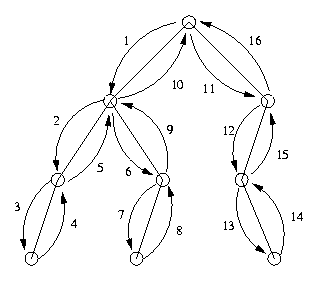
\includegraphics{imagenes/rec2}

El algoritmo recorre el árbol yendo tan abajo como sea posible y luego
retrocediendo cuando sea necesario, haciendo una especie de bosquejo
del árbol cuando los nodos son visitados. Gráficamente, el árbol es
recorrido en la siguiente manera: 

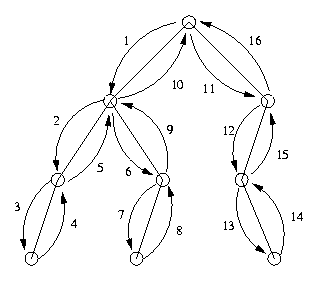
\includegraphics{imagenes/rec22}


\subsubsection{Complejidad}

Suponga que hay d decisiones que deben ser hechas. (En este caso d=n,
el número de columnas que debemos llenar.) Suponga además que hay
C posibilidades para cada decisión. (En este caso c=n también, desde
que cualquiera de las filas podría potencialmente ser elegida.) Entonces
toda la búsqueda tomará tiempo proporcional a $c^{d}$, esto es, una
cantidad exponencial de tiempo. Sin embargo, este esquema requiere
poco espacio: desde que solo lleva registro de tantas decisiones como
las que hay que hacer, requiere solo espacio $O(d)$.


\subsubsection{Problema Ejemplo: Cubrir con Caballos {[}Tradicional{]}}

Coloque tantos caballos como sea posible en un tablero de ajedrez
n x n de tal manera que cada cuadrado sea atacado. Se considera que
un caballo no ataca el cuadrado en el cual está.


\subsection{Búsqueda Primero a lo Ancho(BFS del inglés Breadth First Search)}

En este caso, es deseable tratar con todas las soluciones con solo
k caballos antes de moverse a aquellos con k+1 caballos. Esto es llamado
\emph{búsqueda primero a lo ancho}. La manera usual de implementar
la búsqueda primero a lo ancho es usar una pila de estados: 

\begin{lstlisting}
procesar(estado)
    para cada siguente estado posible desde este estado
        añada a la cola el siguiente estado

buscar()
    añada a la cola el estado inicial
    mientras !vacia(cola)
        estado = conseguir estado de cola
        procesar(estado) 
\end{lstlisting}


Esto es llamado búsqueda primero a lo ancho debido a que busca toda
una fila entera (el ancho) de cada árbol de búsqueda antes de moverse
a la siguiente fila. Para el árbol de búsqueda usado previamente,
la búsqueda primero a lo ancho visita los nodos en este orden: 

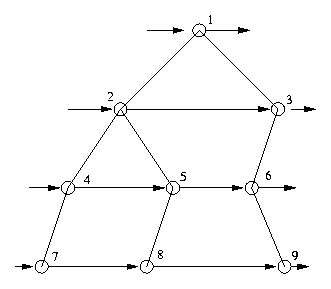
\includegraphics{imagenes/rec3}

Primero visita el nodo tope, luego los nodos en el nivel 1, luego
todos los de nivel 2, y así sucesivamente.


\subsubsection{Complejidad}

Mientras que la búsqueda primero en profundidad requiere espacio proporcional
al número de decisiones (hay n columnas para llenar en el problema
de las n reinas, por lo tanto tomó$O(n)$espacio), la búsqueda primero
a lo ancho requiere espacio exponencial en el número de posibilidades.

Si hay c posibilidades en cada decisión y se han hecho k decisiones,
entonces hay $c^{k}$ tableros posibles que estarán en la cola para
la siguiente ronda. esta diferencia es de gran importancia dadas las
restricciones de algunos ambientes de programación.

\emph{{[}Algunos detalles de porque $c^{k}$: Considere los nodos
en el árbol de recursión. El nivel cero tiene 1 nodo. El primer nivel
tiene $C$ nodos. El siguiente nivel tiene $c^{2}$ nodos, etc. Por
lo tanto, el número total de nodos en el nivel k-ésimo es $c^{k}$.{]}}


\subsection{Busqueda por Profundidad Iterativa(ID)}

Una alternativa para la búsqueda primero en ancho es profundización
iterativa.En lugar de una sola búsqueda primero a lo ancho, corre
D búsquedas primero en profundidad en sucesión, permitiendo que cada
búsqueda vaya una fila más profunda que la anterior. Esto es, la primera
búsqueda solo puede explorar la fila 1, la segunda la fila 2, y así
sucesivamente. Esto \textquotedbl{}simula\textquotedbl{} una búsqueda
primero a lo ancho en costo en tiempo pero ahorrando espacio. 

\begin{lstlisting}
truncated_dfsearch(hnextpos, depth)
    if board is covered
        print solution and exit 

    if depth == 0
        return 

    for i from nextpos to n*n
        put knight at i
        truncated_dfsearch(i+1, depth-1)
        remove knight at i 

dfid_search
    for depth = 0 to max_depth
       truncated_dfsearch(0, depth)
\end{lstlisting}



\subsubsection{Complejidad}

La complejidad en espacio de una profundización iterativa es simplemente
la complejidad de una búsqueda primero en profundidad: $O(n)$. La
complejidad de tiempo, por otro lado, es más compleja. Cada búsqueda
en profundidad truncada, parando en profundidad k toma $c^{k}$ tiempo.
Luego si d es el número máximo de decisiones, la búsqueda en profundidad
primero toma $c^{0}+c^{1}+c^{2}+...+c^{d}$ tiempo.

Si $c=2$, entonces esta suma es $i>c^{d+1}-1$, cerca del doble de
tiempo que lo que hubiera tomado la búsqueda primero en profundidad.
Cuando c es mayor que dos (esto es, cuando hay muchas posibilidades
para cada decisión), la suma es aún menos: la profundización iterativa
no puede tomar más que dos veces el tiempo que la búsqueda primero
a lo ancho hubiera tomado, asumiendo que hay siempre al menos dos
posibilidades para cada elección.


\subsection{¿Cuál usar?}

Una vez que usted ha identificado un problema como un problema de
búsqueda, es importante elegir el tipo adecuado de búsqueda. Aquí
hay algunas cosas para pensar


\subsubsection*{En Resumen}

\begin{longtable}{|c|c|c|l|}
\hline 
Búsqueda & Tiempo & Espacio & Cuando usarla\tabularnewline
\hline 
\hline 
DFS & O(c\textasciicircum{}k) & O(k) & Se debe recorrer el árbol de todas maneras, se conoce el nivel donde
están las respuestas, o usted no está buscando la respuesta menos
profunda.\tabularnewline
\hline 
BFS & O(c\textasciicircum{}d) & O(c\textasciicircum{} d) & Se debe recorrer el árbol de todas maneras, se conoce el nivel donde
están las respuestas, o usted no está buscando la respuesta menos
profunda.\tabularnewline
\hline 
DFS+ID & O(c\textasciicircum{}d) & O(d) & Se quiere hacer BFS, pero no se tiene suficiente espacio, y se puede
gastar en tiempo.\tabularnewline
\hline 
\end{longtable}

$d$es la profundidad de la respuesta

$k$es la profundidad buscada 

$d<=k$

Recuerde las propiedades de orden de cada búsqueda. Si el programa
necesita producir una lista de la solución más corta primero (en términos
de distancia desde el nodo raíz), use búsqueda primero a lo ancho
o de profundización iterativa. Para otros ordenes, la búsqueda primero
en profundidad es la estrategia adecuada. Si no hay suficiente tiempo
para buscar todo el árbol, use el algoritmo que sea más apropiado
para encontrar la respuesta. Si la respuesta se espera en una de las
filas o de los nodos cercanos a la raíz, use búsqueda primero a lo
ancho o de profundidad iterativa. Por el contrario, si se espera que
la respuesta esté en una de las hojas, use la búsqueda más simple
de profundidad primero.

Este seguro de tener las restricciones de espacio en mente. Si la
memoria es insuficiente para mantener la cola para búsqueda primero
a lo ancho pero dispone de tiempo, use profundidad iterativa.


\subsection{Problemas Ejemplo}


\subsubsection*{Cadena Superprima {[}USACO 1994 Ronda Final, adaptado{]}}

Un número es llamado superprimo si es primo y si cada número obtenido
quitando algún número de digítos del lado derecho de la expansión
decimal es primo. Por ejemplo, 233 es superprimo, porque 233, 23,
y 2 son todos primos. Imprima una lista de todos los números superprimos
de longitud n, para n <= 9. El número 1 no es primo.

Para este problema, use búsqueda primero en profundidad, desde que
todas las respuestas van a estar en el nivel n-ésimo (el de más abajo)
de la búsqueda.


\subsubsection*{Paseo de Betsy {[}USACO 1995 Ronda Clasificatoria{]}}

Un pueblo cuadrado ha sido particionado en $n^{2}$ parcelas cuadradas.
La Granja está ubicada en la parcela superior izquierda y el Mercado
está ubicado en la parcela inferior izquierda. Betsy da un paseo a
través del pueblo yendo de la Granja al Mercado caminando a través
de cada parcela exactamente una vez. Escriba un programa que cuente
de cuántas maneras diferentes Betsy puede ir de la Granja al Mercado
para cualquier valor de n <= 6.

Como se requiere el número de soluciones, se debe buscar todo el árbol,
aún si se encuentra rápidamente una solución. Por lo tanto no importa
desde la perspectiva de tiempo si es usado un DFS o un BFS. Como un
DFS toma menos espacio, es la búsqueda de elección para este problema.


\subsubsection*{Udder Travel {[}USACO 1995 Ronda Final; Piele{]}}

La compañía Transportadora de Vacas Udder Travel tiene su centro de
operaciones en la granja A y posee un camión de vacas el cual es usado
para recoger y llevar vacas entre siete granjas A, B, C, D, E, F,
y G. Las distancias (conmutativas) entre las granjas son dadas por
un arreglo. Cada mañana, Udder Travel tiene que decidir, dado un conjunto
de movimientos de vacas, el orden en el cual recoger y llevar las
vacas para minimizar la distancia total recorrida. Aquí están las
reglas:
\begin{itemize}
\item El camión siempre comienza de la central en la granja A y debe devolverse
allí cuando se hayan hecho las entregas del día. 
\item El camión solamente puede llevar una vaca al tiempo.
\item Las ordenes son dadas como pares de letras denotando donde se debe
recoger una vaca seguido de a donde la vaca debe ser llevada.
\end{itemize}
Su trabajo es escribir un programa que, dado cualquier conjunto de
ordenes, determine la ruta más corta que se encargue de todas las
entregas, comenzando y terminando en la granja A.

Como se debe intentar con todas las posibilidades con el propósito
de asegurarse que se encuentra el mejor, todo el árbol debe ser recorrido,
lo cual toma la misma cantidad de tiempo usando DFS o BFS. Desde que
DFS usa mucho menos espacio y es conceptualmente más fácil de implementar,
úselo.


\subsubsection*{Cruzando el Desierto {[}IOI 1992, adaptado{]}}

Los miembros de un grupo de nómadas del desierto están trabajando
juntos para tratar de que uno de ellos atraviese el desierto. Cada
nómada puede llevar cierta cantidad de litros de agua, y cada nómada
toma cierta cantidad de agua por día, pero cada uno puede llevar una
cantidad diferente de agua, y requiere una cantidad diferente de agua.
Dada la capacidad de carga y los requerimientos de agua de cada nómada,
encuentre el mínimo número de nómadas requeridos para que al menos
uno de ellos cruce el desierto.

Todos los nómadas deben sobrevivir, por lo tanto cada nomada que comience
el recorrido o debe regresar en algún punto, cargando suficiente agua
para volver al inicio o debe alcanzar el otro lado del desierto. Sin
embargo, si un nómada tiene un sobrante de agua cuando es tiempo de
regresar, puede repartir ese sobrante entre sus amigos, si sus amigos
pueden cargarla.
\begin{description}
\item [{Análisis:}] Este problema es realmente dos problemas recursivos:
una recursión en el conjunto de nómadas a usar, el otro cuando los
nómadas deben volver. Una búsqueda en profundidad primero con profundización
iterativa trabaja bien aquí para determinar los nómadas requeridos,
tratando primero si uno puede hacerlo por si solo, luego viendo si
dos lo pueden hacer, etc.
\end{description}

\subsubsection*{Cadenas de Adición}

Una cadena de adición es una secuencia de enteros tales que el primer
número es 1, y cada número subsecuente es la suma de algunos dos números
(no necesariamente únicos) que aparecen en la lista antes que él.
Por ejemplo 1 2 3 5 es una cadena de esas, pues 2 es 1+1, 3 es 2+1,
y 5 es 2+3. Encuentre la cadena de mínima longitud que termine con
un número dado.
\begin{description}
\item [{Análisis:}] La Búsqueda primero en profundidad con profundización
iterativa trabaja bien aquí, pues DFS tiene una tendencia de primero
intentar 1 2 3 4 5 ... n, lo cual es realmente malo y la cola llega
a ser muy grande rápidamente para BFS. 
\end{description}

\section{Introducción a Números Binarios}


\subsection{Representando Números Binarios}

Las computadoras trabajan con 1's y 0's; estos son llamados 'bits'.
Un byte es un grupo de 8 bits, como este: 00110101. Una palabra en
mi computadora ('int') es de bytes: 
\begin{lyxcode}
10011010110101011010001010101011.~
\end{lyxcode}
Otras computadoras tienen tamaños diferentes de palabras.

Como puede ver 32 unos y ceros es un poco incómodo de escribir (o
aún leer). Por lo tanto, la gente convencional parte el número en
grupos de 3 o 4 bits:
\begin{lyxcode}
1001.1010.1101.0101.1010.0010.1010.1011

10.011.010.110.101.011.010.001.010.101.011

<-{}-~note~que~el~contador~de~3~comienza~en~la~derecha~
\end{lyxcode}
Estos conjuntos de bits son entonces enviados a dígitos, o cuatro
dígitos por dígito hexadecimal (base 16) o tres dígitos por dígito
octal (base 8). Obviamente, los hexadecimales necesitan algunos nuevos
dígitos (los dígitos decimales solo van de 0 a 9 y necesitamos 6 más).
Actualmente, se usan las letras 'A'..'F' s para los 'dígitos' que
representan 10..15. Aquí está la tabla, la correspondencia es obvia:
\begin{lyxcode}
~~~~OCTAL:~~~~~~~~~~~~~~~~~~~HEXADECIMAL:

~~000~->~0~~100~->~4~~~~~~~0000~->~0~~0100~->~4~~1000~->~8~~1100~->~C

~~001~->~1~~101~->~5~~~~~~~0001~->~1~~0101~->~5~~1001~->~9~~1101~->~D

~~010~->~2~~110~->~6~~~~~~~0010~->~2~~0110~->~6~~1010~->~A~~1110~->~E

~~011~->~3~~111~->~7~~~~~~~0011~->~3~~0111~->~7~~1011~->~B~~1111~->~F
\end{lyxcode}
Por lo tanto ahora podemos escribir las representaciones hexadecimal
y octal de aquellos enteros antes vistos rápidamente con sus notaciones
para C y otros lenguajes:
\begin{lyxcode}
~~~~	1001.1010.1101.0101.1010.0010.1010.1011

~->~~~~~9~~~~A~~~~D~~~~5~~~~A~~~~2~~~~A~~~~B~~-{}->~0x9AD5A2AB

			~~~~	(esto~es~0x~in~delante~del~número~hexadecimal)
\end{lyxcode}
y
\begin{lyxcode}
	~~~~~10.011.010.110.101.011.010.001.010.101.011

~~~~~~2~~~3~~~2~~~6~~~5~~~3~~~2~~~1~~~2~~~5~~~3~->~023265321253

		~~~~~~~~~~~~~~~~~		(esto~es~un~~'0'~numérico~delante)
\end{lyxcode}
El sistema octal es más fácil de escribir rápidamente, pero el hexadecimal
tiene propiedades bonitas de distribuirse fácilmente en bytes (los
cuales son pares de dígitos).


\subsection{Manejando Números Binarios en Programas}

Algunas veces es conveniente trabajar con los bits almacenados en
números en vez de simplemente manejarlos como enteros. Ejemplos de
tales casos incluyen recordar elecciones (cada posición puede ser
un indicador 'si'/'no'), manteniendo registro de banderas de opción
(realmente la misma idea, cada posición de bit es un indicador 'si'/'no'
de la presencia de una bandera), o llevando registro de enteros pequeños
(esto es pares sucesivos de posiciones de bits pueden memorizar números
de 0 a 3). Por supuesto, ocasionalmente los problemas pueden contener
realmente 'cadenas de bits'.

En C/C++ y en otros lenguajes, asignar números binarios es fácil si
usted conoce su representación octal o hexadecimal:
\begin{lyxcode}
i~=~0x9AD5A2AB;~
\end{lyxcode}
o
\begin{lyxcode}
i~=~023265321253;
\end{lyxcode}
Con mayor frecuencia , un conjunto de valores de bit únicos es combinado
para crear un entero de interés. Uno podría pensar que la sentencia
de a continuación haría eso:
\begin{lyxcode}
i~=~0x10000~+~0x100;~
\end{lyxcode}
y lo hará \textendash{} hasta que el bit de signo entre en la película
y el mismo bit sea combinado dos veces:
\begin{lyxcode}
i~=~0x100~+~0x100;
\end{lyxcode}
En ese caso, ocurre un 'acarreo' y entonces i contiene 0x200 en vez
de 0x100 como era probablemente lo deseado. La operación 'or' denotada
en C/C++ y otros como '|' \textendash{} hace la cosa correcta. Combina
bits sucesivos usando estas cuatro reglas:
\begin{lyxcode}
~0|0~->~0

~0|1~->~1

~1|0~->~1

~1|1~->~1
\end{lyxcode}
La operación '|' es llamada 'bitwise or' en C para no ser confundida
con su prima '||' llamada 'or lógico' evalúa el valor aritmético de
su lado izquierdo y, si es falso (exactamente 0), evalúa su lado derecho.
Si cualquier evaluación es no cero, entonces '||' evalúa a verdad
(exactamente 1 en C). Es la regla final la que distingue al operador
'|' del operador '+'. Algunas veces los operadores como estos son
mostrados en una 'tabla de verdad':
\begin{lyxcode}
~|~|~0~~1

-{}-{}-+-{}-{}-{}-{}-{}-

~0~|~0~~1

~1~|~1~~1
\end{lyxcode}
Un '1' aparece solo cuando \textquotedblleft{}ambos\textquotedblright{}
bits de entrada son '1'. Por lo tanto, si uno quiere saber si el bit
0x100 es '1' en un entero, la instrucción if es simple:
\begin{lyxcode}
if~(a~\&~0x100)~\{~printf(\textquotedbl{}yes,~0x100~is~on\textbackslash{}n\textquotedbl{});~\}
\end{lyxcode}
C/C++ (y otros) contienen operadores adicionales, incluyendo el o
'exclusivo' (denotado '\textasciicircum{}') con su tabla de verdad:
\begin{lyxcode}
~\textasciicircum{}~|~0~~1~~~~~~~~~

-{}-{}-+-{}-{}-{}-{}-{}-~~~~~~~~~~

~0~|~0~~1~~~~~~~~~~

~1~|~1~~0
\end{lyxcode}
Se llama al operador 'o exclusivo' algunas veces 'xor\textquotedblright{}
por facilidad de escritura. Xor da un '1' si exactamente {*} una{*}
des sus entradas es uno: la primera o la segunda, pero no las dos.
Este operador es muy útil para 'voltear' bits, cambiándolos de '1'
a '0' o viceversa. Considere esta instrucción:
\begin{lyxcode}
	a~=~a~\textasciicircum{}~0x100;~~~/{*}~same~as~a~\textasciicircum{}=~0x100;~{*}/
\end{lyxcode}
El bit 0z100 cambiará de 0->1 o de 1->0, dependiendo de su valor actual.
Apagar un bit requiere dos operadores. El nuevo es el operador unario
que voltea cada bit en una palabra, creando lo que se llama el 'complemento
bitwise' o simplemente 'complemento' de una palabra. Algunas veces
esto es llamado 'inversión de bits' o simplemente 'inversión' y se
denota por la tilde '\textasciitilde{}'. Aquí hay un ejemplo rápido:
\begin{lyxcode}
char~a,~b;	/{*}~eight~bits,~not~32~{*}/~	

a~=~0x4A;	~/{*}~0100.1010~{*}/~	

b~=~\textasciitilde{}a;	~~~/{*}~flip~every~bit:~1011.0101~{*}/~	

printf(\textquotedbl{}b~is~0x\%X\textbackslash{}n\textquotedbl{},~b);~
\end{lyxcode}
lo cual da algo como: 	
\begin{lyxcode}
b~es~0xB5
\end{lyxcode}
Por lo tanto, si nosotros tenemos uno solo bit encendido (por ejemplo
0x100) entonces \textasciitilde{}0x100 tiene todos los bits prendidos
menos uno: 0xFFFFFEFF (note que la 'E' es el tercer 'digíto' desde
la derecha)

Estos dos operadores se combinan para crear un esquema para borrar
bits:
\begin{lyxcode}
a~=~a~\&~(\textasciitilde{}0x100);	/{*}~borrar~el~bit~0x100~~{*}/~				

~~~~~~~~~~~~~~~~~~/{*}~lo~mismo~que~\&=~\textasciitilde{}0x100;
\end{lyxcode}
como todos los bits menos 1 en \textasciitilde{}0x100 están prendidos,
todos los bits menos el bit 0x100 aparecen en el resultado. Desde
que el bit 0x100 está 'apagado' en \textasciitilde{}0x100, ese bit
se garantiza que es '0' en el resultado. Esta operación es llamada
universalmente un 'enmascarameinto' como 'desmascarar el bit 0x100'.


\subsection{Resumen}

En resumen, estos operadores permiten establecer, borrar, voltear
y verificar cualquier bit o combinación, de bits en un entero:
\begin{lyxcode}
a~|=~0x20;		/{*}~prende~el~bit~bit~0x20~{*}/~		

a~\&=~\textasciitilde{}0x20;	~~~/{*}~apaga~el~~bit~0x20~~{*}/~		

a~\textasciicircum{}=~0x20;		/{*}~voltea~el~~bit~0x20~{*}/~		

if~(a~\&~0x20)~\{~			
\begin{lyxcode}
/{*}~entonces~el~bit~0x20~esta~prendido~~{*}/~		
\end{lyxcode}
\}\end{lyxcode}

\end{document}
